\documentclass[11pt,letterpaper]{article}
\topmargin-2cm
\oddsidemargin0cm
\evensidemargin0cm
\textheight23cm
\textwidth16cm


\usepackage{textcomp}
\usepackage{listings}
\usepackage{amssymb}
\usepackage{amsmath}
\usepackage{url}
\usepackage{graphicx}
\usepackage[all]{xy}
\usepackage{pstricks}
%\usepackage[notref,notcite]{showkeys}

\lstset{xleftmargin=1cm}

\newcommand{\nmax}{n_\mathrm{max}}
\newcommand{\x}{\boldsymbol{x}}
\newcommand{\xh}{\widehat{\boldsymbol{x}}}
\newcommand{\y}{\boldsymbol{y}}
\newcommand{\z}{\boldsymbol{z}}
\newcommand{\zero}{\boldsymbol{0}}
\newcommand{\dd}{\boldsymbol{d}}
\newcommand{\hdd}{\widehat{\dd}}

\newcommand{\bbR}{\mathbb{R}}
\newcommand{\bbC}{\mathbb{C}}
\newcommand{\bbN}{\mathbb{N}}
\newcommand{\bbZ}{\mathbb{Z}}

\newcommand{\et}{\widetilde{e}}

\newcommand{\surface}{\partial D}

\newcommand{\inc}{\mathrm{inc}}

\newcommand{\ri}{\nu}

\newcommand{\ie}{{\em i.e.}}
\newcommand{\eg}{{\em e.g.}}

\setlength{\parindent}{0cm}
\setlength{\parskip}{3ex}

\newtheorem{example}{Example}

\newcommand{\techheading}[1]{%
    \par\vspace{-0.3\parskip}\noindent\hspace{-1cm}\textbf{#1}%
    \par\vspace{-0.5\parskip}\noindent\nopagebreak\ignorespaces}

%\newenvironment{mylisting}{\begin{lstlisting}[language=matlab,basicstyle=\ttfamily,belowskip=-0.3 \baselineskip]}{\end{lstlisting}}

%\newenvironment{mylisting}{\begin{lstlisting}}{\end{lstlisting}}

\lstnewenvironment{matlab}{\lstset{language=matlab,basicstyle=\ttfamily,commentstyle=\ttfamily,belowskip=-0.3 \baselineskip,columns=fullflexible,upquote=true}}{}

\lstnewenvironment{unix}{\lstset{language=bash,basicstyle=\ttfamily,belowskip=-0.4 \baselineskip,columns=fullflexible}}{}

\lstnewenvironment{dos}{\lstset{language=dos,basicstyle=\ttfamily,belowskip=-0.3 \baselineskip,columns=fullflexible}}{}

\lstMakeShortInline[language=matlab,basicstyle=\ttfamily,belowskip=-0.3 \baselineskip]!

\bibliographystyle{plain}

\begin{document}
\title{MieSolver: a Matlab object-oriented Mie series software}


\author{
Stuart C. Hawkins,\\ Department of Mathematics and Statistics,\\Macquarie University, Sydney, NSW 2109, Australia \\
{\tt stuart.hawkins@mq.edu.au}}
\date{}

\maketitle

\begin{abstract}
  We provide a user manual for our
  object-oriented Matlab package
  MieSolver, which provides efficient and easy to use tools
  for simulating wave propagation through a heterogeneous configuration
  of nonidentical circular cylinders.
  MieSolver allows great flexibility in the physical properties
  of each cylinder and the cylinders may have opaque or penetrable cores,
  and an arbitrary number of penetrable layers.
  The solver is based on the Mie series solution and hence is numerically
  stable and highly accurate.
\end{abstract}

\section{Installation  and verification}

\techheading{Download}
Download the CALGO \textit{zip} file and unpack it.

Your system may automatically unpack the archive file for you.
If your system does not do this then you can unpack it
using either 

unzip XXXX.zip

\noindent
where XXXX is the algorithm number
or by opening it with Winzip (Windows).

\techheading{Setting up Matlab}
In the directory \textit{Matlab} there are two subdirectories \textit{Src} and \textit{Drivers}; add both of these to Matlab's search path.

Below we refer to the \textit{Src} directory as the MieSolver root directory.

\techheading{Run example codes}
Several example scripts are included in the \textit{Drivers} directory.
These can be executed by running the following scripts:
\begin{matlab}
mie_example_soft
mie_example_hard
mie_example_robin
mie_example_coated
mie_example_dielectric
\end{matlab}
The figures produced by these examples are included in the Appendix.

We recommend users follow the quick start guide in Section~\ref{sec:start}
to learn more about how to use the package.

\tableofcontents




\section{Introduction}

We describe the use of our object-oriented Matlab software package
MieSolver.
This package provides software tools for simulation of wave scattering
in two dimensions
by circular obstacles.
Heterogeneous configurations containing many nonidentical 
obstacles with various material properties, with and without penetrable layers,
can be simulated.
The two dimensional wave scattering problem arises in models for propagation
of acoustic, elastic and electromagnetic waves in domains
containing parallel circular cylinders and we refer to the accompanying
paper~\cite{mietoms}
for further details and references.

The object-oriented structure of our package facilitates easy
description of the scattering problem,
including the incident wave and the
obstacles in a configuration, even for
large heterogeneous configurations of nonidentical obstacles.
As demonstrated in Section~\ref{sec:start}, only a few lines of simple
code are required to setup and solve a wave scattering simulation with a
single scatterer.
Examples in Section~\ref{sec:examples} show that simulations with multiple
scatterers and layered scatterers are similarly easy to code.

Our code is based on the well known Mie series,
which has been widely described in books,
including~\cite{bohren,rother,hulst:light}.
For further references to the extensive literature on the Mie series for
the two dimensional
scattering problem we refer to~\cite{mietoms}.
It is well known that the Mie series yields highly accurate solutions.
In~\cite{mietoms} we demonstrate eight digit accuracy of our code in 
extensive numerical experiments for a wide range of configurations with
varying numbers of obstacles and various material parameters.

This article includes the minimal mathematical details required to
use the package and understand
the underlying algorithm.
For complete mathematical details we ask the user of this manual
to refer to~\cite{mietoms}.
\textit{We request that any publications that make
  use of our MieSolver package cite
our accompanying paper~\cite{mietoms}.}

\paragraph{A note on position vectors in MieSolver}

In our MieSolver code, and in this manual,
we represent real valued vectors (such as position vectors)
$(x,y)^T \in \bbR^2$  by 
complex numbers $x+yi$.

\section{Quick start guide}
\label{sec:start}

In this section we describe how to setup, simulate and visualise
the scattered field and far field induced by a plane wave interacting
with a cylinder comprising a sound-soft core and a penetrable layer.

First we set up the sound-soft
scatterer core (with radius 0.5 and centre at the origin)
using
\begin{matlab}
s = scatterer(0,0.5,'SOFT');
\end{matlab}
Then we add the penetrable layer (with outer radius 1 and refractive
index 1.5) using
\begin{matlab}
s.addCoating(1,1.5);
\end{matlab}

Next we set up the incident plane wave (with wavenumber 5 and direction
$\dd = (\cos \theta,\sin \theta)^T$ for $\theta = \pi/2$) using
\begin{matlab}
p = plane_wave(pi/2,5);
\end{matlab}

Next we setup the solver, set the tranmsission type to TE,
add the scatterer,
and solve to find the scattering coefficients.
\begin{matlab}
m = MieSolver(p);
m.transmissionTE();
m.addScatterer(s);
m.solve();
\end{matlab}

We visualise the total field (using the default plotting region) using
\begin{matlab}
m.visualiseTotalField()
\end{matlab}
The output is shown in Figure~\ref{fig:quick-start}.
To modify the plotting region please see the detailed instructions in
Section~\ref{sec:mieproblem}.

We visualise the far field using
\begin{matlab}
m.visualiseRcs()
\end{matlab}
The output is shown in Figure~\ref{fig:quick-start}.

\begin{figure}
  \centering
  \begin{tabular}{cc}
    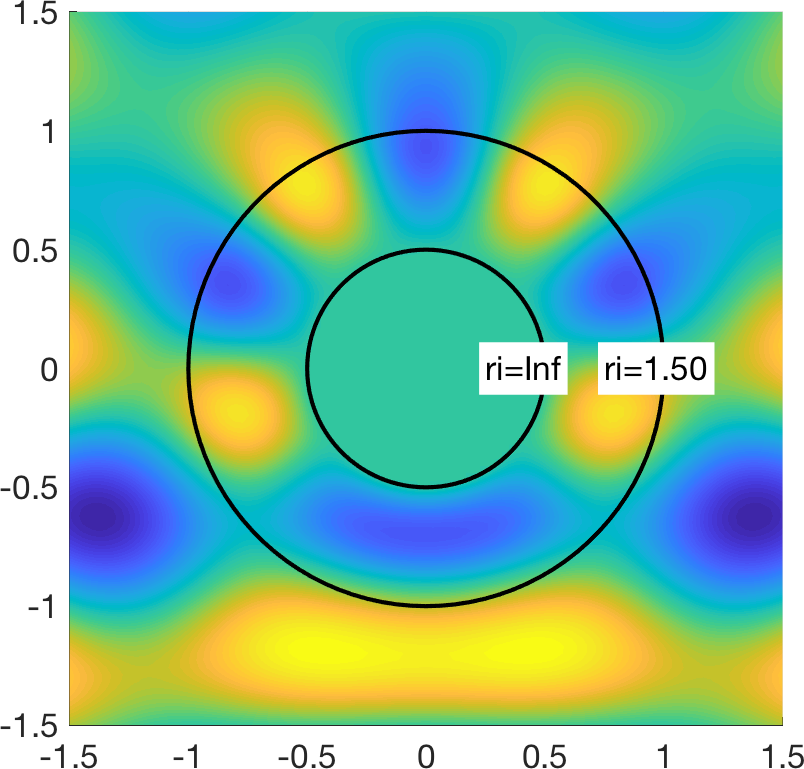
\includegraphics[height=6cm]{quick_start_total_field}
    &
    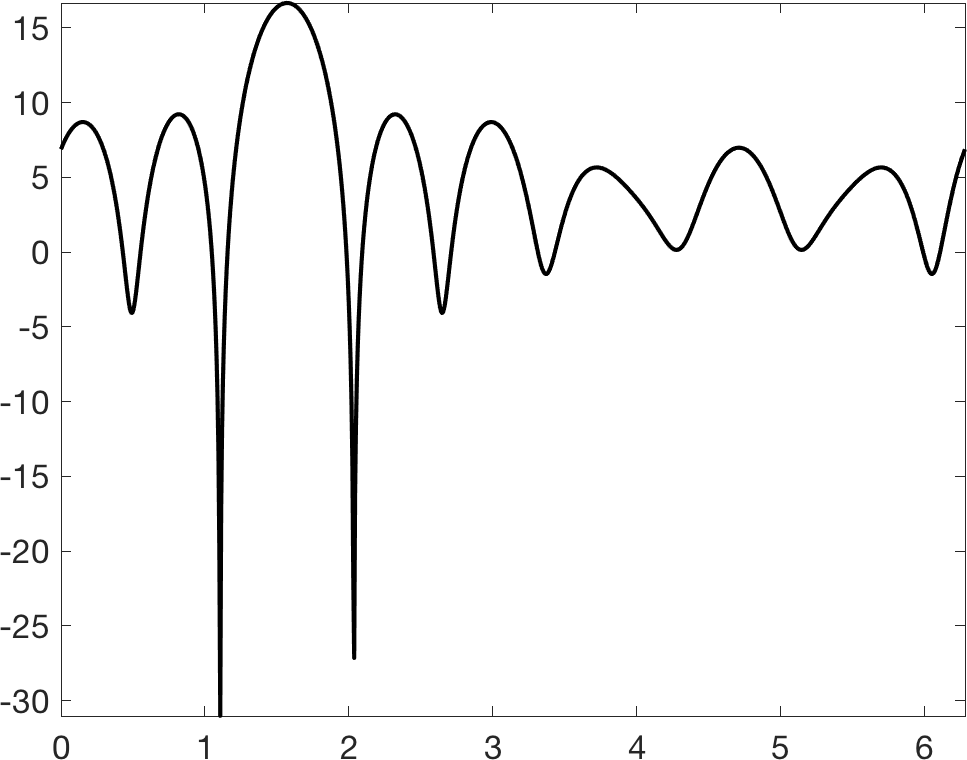
\includegraphics[height=6cm]{quick_start_far_field}
  \end{tabular}
  \caption{\label{fig:quick-start}
    Visualisations of the total field (left) and cross section (right)
    of a cylinder with a sound-soft core and a penetrable layer
    produced using the code in 
    the Quick Start Guide (Section~\ref{sec:start}).}
\end{figure}

\section{Mathematical Model}
\label{sec:model}

\techheading{Overview}
The MieSolver package solves the two dimensional Helmholtz equation,
which models propagation of three dimensional waves through a domain
containing vertical cylinders.
In the two dimensional Helmholtz model the cylinders are represented by
their two dimensional cross sections.
Henceforth we use the term ``scatterer'' to describe the two dimensional
cross sections of the cylinders.

\techheading{Scatterer description}
We begin by briefly describing the scattering problem for the case of a
single circular scatterer centred at the origin.
We assume that the scatterer comprises a homogeneous core
with radius $r_1$ surrounded by $N-1$ homogeneous annular layers
with outer radii $r_2,\dots,r_N$ satisfying
\begin{displaymath}
r_1 < r_2 < \dots < r_N.
\end{displaymath}
(The case in which the core is not surrounded by
any layers satisfies this description with $N=1$.)
The core is then
\begin{displaymath}
D_1 = B(\zero,r_1)
\end{displaymath}
where $B(\x,r)$ denotes the ball or radius $r$ centred at $\x$.
The annular layers are 
\begin{displaymath}
  D_j = B(\zero,r_j) \setminus B(\zero,r_{j-1}),
  \qquad \mbox{for $2 \leq j \leq N$}.
\end{displaymath}
It is convenient to denote the outer domain
\begin{displaymath}
D_{N+1} = \bbR^2 \setminus B(\zero,r_N).
\end{displaymath}

\techheading{PDEs and boundary conditions}
The scatterer
$D = D_1 \cup \cdots \cup D_N$
is illuminated by an incident wave $u^\inc$ with wavenumber $k$,
which induces a
field $u_j$ in each of the domains $D_j$ for $j=1,\dots,N+1$.
(If the core is opaque then it is convenient to set the field in the core,
$u_1 = 0$.)
The induced fields
satisfy the two dimensional Helmholtz equation
\begin{equation}
  \label{eq:helmholtz}
  \triangle u(\x) + (\ri_j k)^2 u(\x) = 0, \qquad \x \in D_j,
\end{equation}
where $\ri_j$ denotes the refractive index in $D_j$
for $j=1,\dots,N$ and,
without loss of generality, we may fix the refractive
index in the exterior domain $D_{N+1}$ to be $\ri_{N+1}=1$.

The induced field $u_{N+1}$ in the exterior domain $D_{N+1}$ is also 
known as the scattered field, and is required to satisfy
the Sommerfeld radiation condition~\cite[Equation~(3.85)]{colton:inverse}
\begin{equation}
  \label{eq:radiation-condition}
  \lim_{|\x|\to \infty} \sqrt{|\x|} \left( \frac{\partial u_{N+1}}{\partial \x}(\x)
  - i k u(\x) \right) = 0
\end{equation}
uniformly as $|\x| \to \infty$.


On the interface between the
penetrable domains $D_j$ and $D_{j+1}$ for $j=1,\dots,N$ we
apply transmission boundary conditions
\begin{align}
  \label{eq:transmission-inner}
  \begin{split}
    u_{j}(\x) & = u_{j+1}(\x), \qquad \mbox{for $\x \in S_j$},\\
    \alpha_j \frac{\partial u_j}{\partial n}(\x) & =
    \alpha_{j+1}\frac{\partial u_{j+1}}{\partial n}(\x),    
     \qquad \mbox{for $\x \in S_j$},
  \end{split}
\end{align}
where $S_j = S(\zero,r_j)$ is the interface between 
$D_j$ and $D_{j+1}$,
and $S(\x,r)$ denotes the sphere centred at $\x$ and with radius $r$.
The parameters $\alpha_j$ and $\alpha_{j+1}$ are transmission parameters
that we describe
below.


If the core is penetrable with refractive index
$\ri_1$ then the incident wave induces
a field $u_1$ in $D_1$, which also satisfies~\eqref{eq:helmholtz}.\
In this case we
apply transmission boundary conditions
\begin{align}
  \label{eq:transmission-core}
  \begin{split}
    u_{1}(\x) & = u_{2}(\x), \qquad \mbox{for $\x \in S_1$},\\
    \alpha_1 \frac{\partial u_1}{\partial n}(\x) & =
    \alpha_2 \frac{\partial u_{2}}{\partial n}(\x),    
     \qquad \mbox{for $\x \in S_1$},
  \end{split}
\end{align}
where $S_1 = S(\zero,r_1)$.
Here $\alpha_1$ and $\alpha_{2}$ are transmission parameters that we describe
below.

If the core is opaque then a Neumann, Dirichlet or Robin boundary condition
is applied on $S_1$ depending on the material properties of the core.
For example, if the core is sound soft then we apply the boundary
condition
\begin{equation}
  \label{eq:soft}
  u_2(\x) = 0, \qquad \mbox{for $\x \in S_1$}.
\end{equation}
If the core is sound hard then we apply the boundary condition
\begin{equation}
  \label{eq:hard}
  \frac{\partial u_2}{\partial n}(\x) = 0, \qquad \mbox{for $\x \in S_1$}.
\end{equation}
Alternatively we may apply the Robin boundary condition
\begin{equation}
  \label{eq:robin}
   \frac{\partial u_2}{\partial n} + i \mu u_2(\x) = 0, \qquad \mbox{for $\x \in S_1$},
\end{equation}
where $\mu \in \bbC$ is a fixed parameter.

In many applications the quantity of interest is the far field
\begin{equation}
  \label{eq:far-field}
  u^\infty(\xh) = \lim_{|\x|\to \infty} \sqrt{|\x|} e^{-ik|\x|} u_{N+1}(\x),
\end{equation}
or the associated cross section (in decibels)
\begin{equation}
  \label{eq:rcs}
  \sigma^{\mathrm{dB}}(\xh) = 10 \log_{10} 2 \pi |u^\infty(\xh)|^2.
\end{equation}
Here $\xh$ is a unit vector that corresponds to the direction of
observation.

\techheading{Transmission parameters}
The transmission parameters
in~\eqref{eq:transmission-inner}
and~\eqref{eq:transmission-core} can be specified by the user
as functions of the refractive index or individually for each core.
Alternatively, default parameters can be chosen
for acoustic scattering or
electromagnetic scattering (TE and TM polarisation) problems.
The procedures for setting the transmission parameters are
given in Section~\ref{sec:class-scatterer}.

\techheading{Solution representation}
A detailed description of the method of solution is given in~\cite{mietoms}.
The induced field in the
core is represented as
\begin{equation}
  \label{eq:expansion-core}
  u_1(\x) = \sum_{n=-\infty}^\infty a^{(1)}_n J_{|n|}(\ri_1 k r) e^{i n \theta}
\end{equation}
for expansion coefficients $(a^{(1)}_n)_{n \in \bbZ}$.
Here we use polar coordinates $\x = 
(r \cos \theta,r \sin \theta)^T$,
and $J_n$ denotes the Bessel function of order $n$.
Similarly, we represent the induced field in each annular layer as
\begin{equation}
  \label{eq:expansion-layers}
  u_j(\x) = \sum_{n=-\infty}^\infty a^{(j)}_n J_{|n|}(\ri_j k r) e^{i n \theta}
  + \sum_{n=-\infty}^\infty b^{(j)}_n H^{(1)}_{|n|}(\ri_j k r) e^{i n \theta},
%  \qquad \mbox{for $2 \leq j \leq N$},
\end{equation}
for $2 \leq j \leq N$,
with expansion coefficients $(a^{(j)}_n)_{n \in \bbZ}$
and $(b^{(j)}_n)_{n \in \bbZ}$.
Here $H_n^{(1)}$ denotes the Hankel function of the first kind of order $n$.
We represent the induced field in the exterior as
\begin{equation}
  \label{eq:expansion-exterior}
  u_{N+1}(\x) = 
  \sum_{n=-\infty}^\infty b^{(N+1)}_n H^{(1)}_{|n|}(k r) e^{i n \theta}
\end{equation}
for expansion coefficients
$(b^{(N+1)}_n)_{n \in \bbZ}$.
This expansion automatically satisfies the radiation 
condition~\eqref{eq:radiation-condition}.

For several important types of incident field, such as plane waves
and point sources, the incident field in the exterior has the expansion
\begin{equation}
  \label{eq:expansion-incident}
  u^\inc(\x) = 
  \sum_{n=-\infty}^\infty a^{(N+1)}_n J_{|n|}(k r) e^{i n \theta}
\end{equation}
with known coefficients $(a^{(N+1)}_n)_{n \in \bbZ}$.
For plane waves and point sources an analytical expression
is available for the coefficients~\cite[Equation~(8)]{mietoms}.

\techheading{Numerical determination of coefficients}
In practice the infinite series 
in~\eqref{eq:expansion-core}--\eqref{eq:expansion-incident}
must be truncated.
In our algorithm we replace summation for $n=-\infty,\dots,\infty$
by summation for $n = -\nmax,\dots,\nmax$ where
\begin{equation}
  \label{eq:wiscombe}
  \nmax = \mathrm{ceil} (n^*), \qquad
n^* = 
  \left\{ \begin{array}{lll}
  x + 1 + 4x^{1/3}, & \quad & \mbox{for $x \leq 8$},\\
  x + 2 + 4.05 \, x^{1/3} & \quad & \mbox{for $8<x<4200$},\\
  x + 2 + 4x^{1/3} & \quad & \mbox{otherwise}.
\end{array} \right.
\end{equation}
Here $x=\pi s = k r_N$ where $s$ is the diameter of the scatterer
in wavelengths,
\begin{equation}
  \label{eq:size}
  s = \frac{2r_{N}}{\lambda} = \frac{k r_N}{\pi}.
\end{equation}
Here $\lambda = 2\pi/k$ denotes the wavelength.
This choice for $\nmax$ is based on 
a formula for the analogous truncation parameter for
Mie scattering by spheres chosen by
Wiscombe~\cite{wiscombe:mie} to give about eight digits accuracy.

Substituting the trucated 
series~\eqref{eq:expansion-core}--\eqref{eq:expansion-exterior}
into the boundary 
conditions~\eqref{eq:transmission-inner}
and~\eqref{eq:transmission-core}--\eqref{eq:robin} yields
a linear system for the unknown coefficients.
The matrix in the linear system
has a block structure with roughly two blocks for each layer
(the exact number depends on the material properties of the core).
Each block is a $(2\nmax +1) \times (2 \nmax+1)$ diagonal matrix.
Therefore it is efficient to assemble the system matrix using Matlab's 
!sparse! function and solve the linear system using Matlab's sparse direct
solver !backslash!.
We refer to~\cite{mietoms} for full details.

%If 
%\begin{displaymath}
%J_n(\nu_j kr) = 0, \qquad J_n(\nu_{j-1} kr) = 0
%\end{displaymath}
%or
%\begin{displaymath}
%J'_n(\nu_j kr) = 0, \qquad J'_n(\nu_{j-1} kr) = 0
%\end{displaymath}
%then the $n$th regular 
%wavefunction in~\eqref{eq:expansion-inner} is a
%Dirichlet of Neumann
%eigenfunction of $D_j$ and the corresponding coefficient $a_n$ is 
%not uniquely defined.

\techheading{Multiple scatterers}
In the case of scattering by a configuration containing $M$ scatterers
with centres $\x_1,\dots,\x_M$
we describe
each scatterer as above, with appropriate modification of the
centres from $\zero$ to $\x_j$ for $j=1,\dots,M$.

Each scatterer contributes its own component of the
form~\eqref{eq:expansion-exterior} to the scattered field in the exterior,
so that the scattered field in the exterior
is given by
\begin{equation}
  \label{eq:expansion-multiple}
  u(\x) = \sum_{j=1}^M 
  \sum_{n=-\infty}^\infty b^{(j,N_j+1)}_n H^{(1)}_{|n|}(k r_j) e^{i n \theta_j}
\end{equation}
where we use polar coordinates
$\x-\x_j = (r_j \cos \theta_j,r_j \sin \theta_j)^T$
\ie{} polar coordinates for $\x$ with local origin $\x_j$.
Here $b^{(j,N_j+1)}_n$ are the expansion coefficients
from~\eqref{eq:expansion-exterior}
on the $j$th scatterer
(and we assume the $j$th scatterer has $N_j$ domains).
The interior fields inside each scatterer are precisely as described above
for the single scatterer case, after appropriate modification of the origin
for the local polar coordinates.

\part{The MieSolver classes}
\label{part:core}

\section{The \texttt{scatterer} class}
\label{sec:class-scatterer}

A MieSolver scatterer comprises a  homogeneous core
and may contain further homogeneous layers.
%with radius $r_1$ surrounded by $N-1$ homogeneous annular layers
%with outer radii $r_2,\dots,r_N$ satisfying
%\begin{displaymath}
%r_1 < r_2 < \dots < r_N.
%\end{displaymath}
A scatterer is built up from the core by adding layers.

\techheading{Instantiation}
The !scatterer! class represents a scatterer
with a core.
An instance of the !scatterer! class with a sound-soft core
(\ie{} a homogeneous Dirichlet boundary condition)
is created using
\begin{matlab}
S = scatterer(x,r,'SOFT');
\end{matlab}
where !x! is the the centre of the scatterer and !r! the radius of the core.

Instances of the !scatterer! class with
sound-hard (\ie{} a homogeneous Neumann boundary condition),
Robin 
or penetrable cores are created similarly, using
\begin{matlab}
S = scatterer(x,r,'HARD');

S = scatterer(x,r,'ROBIN');

S = scatterer(x,r,'DIELECTRIC');
\end{matlab}
where !x! is the the centre of the scatterer and !r! the radius of the core.

In the Robin case, the parameter $\mu$ in~\eqref{eq:robin} will subsequently
need to be set using the !setRobinParameter! method before the scattered
field can be computed.
Alternatively the Robin parameter can be set at the time of instantiation 
using
\begin{matlab}
S = scatterer(x,r,'ROBIN',mu);
\end{matlab}
where !mu! is the value of the Robin parameter.

In the case of a penetrable core, the 
refractive index $\nu$ of the core will subsequently
need to be set using the !setRefractiveIndex! method before the scattered
field can be computed.
Alternatively the refractive index can be set at the time of instantiation 
using
\begin{matlab}
S = scatterer(x,r,'DIELECTRIC',nu);
\end{matlab}
where !nu! is the value of the refractive index in the core.

For acoustic scattering problems,
the density $\rho$ of the core will subsequently
need to be set using the !setDensity! method before the scattered
field can be computed.
Alternatively the density can be set at the time of instantiation 
using
\begin{matlab}
S = scatterer(x,r,'DIELECTRIC',nu,rho);
\end{matlab}
where !nu! is the value of the refractive index in the core
and !rho! is the density of the core.


\techheading{Adding a layer}
A penetrable layer is added to the outside of the scatterer using
\begin{matlab}
S.addCoating(r,nu);
\end{matlab}
where !r! is the outer radius of the layer and !nu! is the refractive
index of the layer.

For acoustic scattering problems
a penetrable layer is added to the outside of the scatterer using
\begin{matlab}
S.addCoating(r,nu,rho);
\end{matlab}
where !r! is the outer radius of the layer, !nu! is the refractive
index of the layer
and !rho! is the density of the layer.

\techheading{Setting the refractive index}
The refractive index in each domain $D_j$ can be modified.
For example,
\begin{matlab}
S.setRefractiveIndex(j,nu)
\end{matlab}
sets the refractive index of domain !j! to !nu!.

If the scatterer has no coatings then
\begin{matlab}
S.setRefractiveIndex(nu)
\end{matlab}
sets the refractive index of the core to !nu!.

\techheading{Setting the density}
The density in each domain $D_j$ can be modified.
For example,
\begin{matlab}
S.setDensity(j,rho)
\end{matlab}
sets the density of domain !j! to !rho!.

If the scatterer has no coatings then
\begin{matlab}
S.setDensity(rho)
\end{matlab}
sets the density of the core to !rho!.

\techheading{Setting the Robin parameter}
If the core has a Robin boundary condition then the
Robin parameter~$\mu$ in~\eqref{eq:robin} is set using
\begin{matlab}
S.setRobinParameter(mu);
\end{matlab}
where !mu! is the value of the Robin parameter.

\techheading{Getting the Robin boundary condition parameter}
The Robin boundary condition parameter $\mu$ in~\eqref{eq:robin}
of the core is obtained using
\begin{matlab}
mu = S.getRobinParameter()
\end{matlab}
If the core does not have a Robin boundary condition then
this method returns !mu = Inf!.

\techheading{Getting the refractive index}
The refractive indices of the domains comprising !S! are obtained
using
\begin{matlab}
nu = S.getRefractiveIndex()
\end{matlab}
Here !nu! is a vector and !nu(j)! contains the refractive index of 
the !j!th domain.
The entry !nu(end)! contains the refractive index of the exterior domain.
If the core is opaque then !nu(1)! is !Inf!.

The refractive index of the !j!th domain is obtained using
\begin{matlab}
nu = S.getRefractiveIndex(j)
\end{matlab}
If the scatterer has no coatings then
\begin{matlab}
nu = S.getRefractiveIndex()
\end{matlab}
returns the refractive index of the core.
If the core is opaque then the result is !nu = Inf!.

\techheading{Getting the density}
The densities of the domains comprising !S! are obtained
using
\begin{matlab}
rho = S.getDensity()
\end{matlab}
Here !rho! is a vector and !rho(j)! contains the density of
the !j!th domain.
The entry !rho(end)! contains the density of the exterior domain.
If the core is opaque then !rho(1)! is !Inf!.

The density of the !j!th domain is obtained using
\begin{matlab}
rho = S.getDensity(j)
\end{matlab}
If the scatterer has no coatings then
\begin{matlab}
rho = S.getDensity()
\end{matlab}
returns the density of the core.
If the core is opaque then the result is !rho = Inf!.

\techheading{Getting the radius of the scatterer}
The radius !r! of the scatterer !S! is obtained using
\begin{matlab}
r = S.getRadius()
\end{matlab}

\techheading{Getting the centre of the scatterer}
The centre !x! of the scatterer !S! is obtained using
\begin{matlab}
x = S.getCentre()
\end{matlab}

\techheading{Getting the acoustic size of the scatterer}
The acoustic size $s$ in~\eqref{eq:size} is obtained using
\begin{matlab}
s = S.getSize(wavenumber)
\end{matlab}
where !wavenumber! is the wavenumber.

\techheading{Visualising the scatterer}
The scatterer is visualised in a 2D figure using
\begin{matlab}
S.show()
\end{matlab}
The linetype for the visualisation can be specified using \eg{}
\begin{matlab}
S.show('k-')
\end{matlab}
The default visualisation includes labels showing the refractive index
of each domain. These labels can be omitted using \eg{}
\begin{matlab}
S.show('k-',0)
\end{matlab}
or
\begin{matlab}
S.show([],0)
\end{matlab}

\section{The \texttt{MieSolver} class}
\label{sec:mieproblem}

The scattering problem described in Section~\ref{sec:model} is setup
and solved using the !MieSolver! class.

\techheading{Instantiation}
A !MieSolver! is constructed using an incident field
of class !incident! and
and one or more scatterers described using objects of class !scatterer!.
An instance of the !MieSolver! class is created using
\begin{matlab}
  P = MieSolver(inc);
\end{matlab}
where !inc! is an object of class !incident!.
The object !P! has no scatterers associated with it and scatterers
must be subsequently added
using the !addScatterer! method
before the induced field can be computed.

Alternatively, one or more scatterers can be added at the time of
instantiation using
\begin{matlab}
P = MieSolver(inc,S);
\end{matlab}
or, for many scatterers,
\begin{matlab}
P = MieSolver(inc,S1,S2,...);
\end{matlab}
where !S!, !S1!, !S2! are objects of class !scatterer!.
The scatterers can also be specified in a cell array,
for example,
\begin{matlab}
P = MieSolver(inc,{S1,S2});
\end{matlab}

\techheading{Setting explicit transmission boundary condition parameters}
To use acoustic scattering type
transmission parameters, specified using the density in each
domain, use the command
\begin{matlab}
P.transmissionAcoustic()
\end{matlab}
In particular the parameter $\alpha_j$
in the transmission
conditions~\eqref{eq:transmission-inner}
and~\eqref{eq:transmission-core} is then given by
\begin{displaymath}
\alpha_j = \frac{1}{\rho_j}
\end{displaymath}
where $\rho_j$ is the density in the $j$th domain.

Note: this option allows each transmission parameter to be specified
explicitly (in terms of its reciprocal).

\techheading{Setting transverse electric (TE)
transmission boundary condition parameters}
To use TE type transmission parameters use the command
\begin{matlab}
P.transmissionTE()
\end{matlab}
In particular the parameter $\alpha_j$
in the transmission
conditions~\eqref{eq:transmission-inner}
and~\eqref{eq:transmission-core} is then given by
\begin{displaymath}
\alpha_j = 1.
\end{displaymath}

\techheading{Setting transverse magnetic (TM)
transmission boundary condition parameters}
To use TM type transmission parameters use the command
\begin{matlab}
P.transmissionTM()
\end{matlab}
In particular the parameter $\alpha_j$
in the transmission
conditions~\eqref{eq:transmission-inner}
and~\eqref{eq:transmission-core} is then given by
\begin{displaymath}
\alpha_j = \frac{1}{\nu_j^2}
\end{displaymath}
where $\nu_j$ is the refractive index in the $j$th domain.

\techheading{Setting custom transmission boundary condition parameters}
To use 
custom transmission parameters specified as a function of
refractive index, use the command
\begin{matlab}
P.transmissionCustom(f)
\end{matlab}
where !f! is a function of one variable.
In particular the parameter $\alpha_j$
in the transmission
conditions~\eqref{eq:transmission-inner}
and~\eqref{eq:transmission-core} is then given by
\begin{displaymath}
\alpha_j = f(\nu_j).
\end{displaymath}
For example, transverse electric (TE) type transmission conditions are
specified using
\begin{matlab}
f = @(nu) 1/nu^2;
\end{matlab}


\techheading{Adding a scatterer}
A scatterer is added using
\begin{matlab}
P.addScatterer(S)
\end{matlab}
where !S! is an object of class !scatterer!.

\techheading{Getting a scatterer}
The !j!th scatterer is obtained using
\begin{matlab}
S = P.getScatterer(j)
\end{matlab}

\techheading{Adjusting the truncation parameter}
The truncation parameter $\nmax$ in Section~\ref{sec:model} is chosen
automatically for each scatterer
to give about eight digits accuracy in the computed
solution using~\eqref{eq:wiscombe}.
This truncation parameter may be adjusted to increase the accuracy.
The truncation parameter is incremented by !m! using
\begin{matlab}
P.incrementNmax(m)
\end{matlab}
This method must be used before the !solve! method.
If the !incrementNmax! method is used more than once then its effects
will be compounded.

\techheading{Getting the truncation parameter}
The truncation parameter $\nmax$ in Section~\ref{sec:model} is obtained
using
\begin{matlab}
n = P.getNmax()
\end{matlab}
Here !n! is a vector and !n(j)! containes the truncation parameter of the
!j!th scatterer.

The truncation parameter for the !j!th scatterer is obtained using
\begin{matlab}
n = P.getNmax(j)
\end{matlab}

\techheading{Computing the induced field coefficients}
The coefficients of the induced fields described in Section~\ref{sec:model}
are computed using
\begin{matlab}
P.solve()
\end{matlab}
This method must be called before the induced field can be computed or
visualised.

\techheading{Getting the induced field}
The induced field described in Section~\ref{sec:model}
is obtained at points !x! using
\begin{matlab}
u = P.getInducedField(x);
\end{matlab}
where !x! is an array of complex numbers representing position vectors.
If !x(j)! lies inside the core of any scatterer then !u(j) = 0!.

\techheading{Getting the total field}
The total field described in Section~\ref{sec:model}
is obtained at points !x! using
\begin{matlab}
u = P.getTotalField(x);
\end{matlab}
where !x! is an array of complex numbers representing position vectors.
If !x(j)! lies inside the core of any scatterer then !u(j) = 0!.

\techheading{Getting the far field}
The far field~\eqref{eq:far-field}
is obtained at points !xh! using
\begin{matlab}
u = P.getFarField(x);
\end{matlab}
where !x! is an array of complex numbers representing position vectors
and !xh = x./abs(x)!.
The points in !xh! lie on the unit circle and represent observation
directions.

\techheading{Getting the Cross Section in decibels}
The cross section~\eqref{eq:rcs}
is obtained at points !xh! using
\begin{matlab}
u = P.getRcs(x);
\end{matlab}
where !x! is an array of complex numbers representing position vectors
and !xh = x./abs(x)!.
The points in !xh! lie on the unit circle and represent observation
directions.

\techheading{Visualising the total field}
The total field is visualised using
\begin{matlab}
P.visualiseTotalField()
\end{matlab}
The figure shows the real part of the total field over a default
rectangular plotting region.

To plot the total field over a custom plotting region
$[\texttt{a},\texttt{c}] \times [\texttt{b},\texttt{d}]$
use
\begin{matlab}
P.visualiseTotalField([a+bi,c+di])
\end{matlab}
The visualisation uses about 10 points per wavelength.
If the grid size exceeds $400 \times 400$ then the visualisation
will be cancelled unless the !-f! override described below is used.

Additional options can be specified using a string !opts!
\begin{matlab}
P.visualiseTotalField([a+bi,c+di],opts)
\end{matlab}
Supported options are:
\begin{itemize}
\item[\texttt{-f}] overrides the $400 \times 400$ grid size restriction.
\item[\texttt{abs}] plots the absolute value of the total field.
\end{itemize}
      
\techheading{Visualising the total field}
The cross section~\eqref{eq:rcs} is visualised using
\begin{matlab}
P.visualiseRcs()
\end{matlab}
The linestyle may additionally be specified \eg{}
\begin{matlab}
P.visualiseRcs('r-')
\end{matlab}
to plot with a solid red line.

\section{The \texttt{incident} class}

Incident fields are represented by the !incident! class.
The !incident! class is an abstract class and two child classes
!plane_wave! and !point_source! are provided.

\techheading{Evaluating an incident field}
An incident field !p! is evaluated at points !z! using
\begin{matlab}
u = p.evaluate(z);
\end{matlab}
Here !z! is an array of complex numbers representing position vectors.

\techheading{Evaluating the gradient of an incident field}
The gradient of an incident field !p! is evaluated at points !z! using
\begin{matlab}
[dx,dy] = p.evaluateGradient(z);
\end{matlab}
Here !z! is an array of complex numbers representing position vectors.
The outputs !dx! and !dy! are the first and second components of
the gradient of the incident field.

\techheading{Obtaining wavefunction expansion coefficients}
The wavefunction expansion coefficients of the incident wave
in~\eqref{eq:expansion-incident}
are given by
\begin{matlab}
cof = p.get_coefficients(x,nmax);
\end{matlab}
where !x! is the expansion centre and !nmax! is the truncation
parameter.

\techheading{Addition and scalar multiplication}
Two objects !p! and !q! of class !incident! can be added using
\begin{matlab}
s = p + q;
\end{matlab}
and substracted using
\begin{matlab}
s = p - q;
\end{matlab}

An object !p! of class !incident! can be multiplied by a scalar using \eg{}
\begin{matlab}
s = 3 * p;
\end{matlab}

\techheading{Incident plane waves}
An incident plane wave
\begin{equation}
  \label{eq:plane-wave}
  u^{\inc}(\x) = e^{i k \x \cdot \hdd}
\end{equation}
with direction specified by the
unit vector $\hdd = (\cos \theta, \sin \theta)^T$
and wavenumber $k$ is represented by the
!plane_wave! class.
An instance of the !plane_wave! class is created using
\begin{matlab}
p = plane_wave(theta,wavenumber);
\end{matlab}
where !theta! is the angle specifying the incident direction
and !wavenumber! is the wavenumber.

\techheading{Incident point sources}
An incident point source
\begin{equation}
  \label{eq:point-source}
  u^{\inc}(\x) = \frac{i}{4} H^{(1)}_0(k |\x - \x_0|)
\end{equation}
with source location $\x_0$
and wavenumber $k$ is represented by the
!point_source! class.
An instance of the !point_source! class is created using
\begin{matlab}
p = point_source(x0,wavenumber);
\end{matlab}
where !x0! is a complex number representing the source location and
and !wavenumber! is the wavenumber.

\section{Examples}
\label{sec:examples}

The solution procedure in the Quick Start Guide (Section~\ref{sec:start})
is independent of the particular configuration of cylinders.
Here we give some examples of how to set up particular configurations.

\techheading{Single sound-soft cylinder (homogeneous Dirichlet BC)}
To setup an instance of the !MieSolver! class for
a single sound-soft cylinder with centre !x! and radius !r!
\begin{matlab}
s = scatterer(x,r,'SOFT');
m = MieSolver(inc,s);
\end{matlab}
where !inc! is of class !incident!.

\techheading{Single sound-hard cylinder (homogeneous Neumann BC)}
To setup an instance of the !MieSolver! class for
a single sound-hard cylinder with centre !x! and radius !r!
\begin{matlab}
s = scatterer(x,r,'HARD');
m = MieSolver(inc,s);
\end{matlab}
where !inc! is of class !incident!.

\techheading{Single absorbing cylinder (homogeneous Robin BC)}
To setup an instance of the !MieSolver! class for
a single absorbing cylinder with centre !x!, radius !r!
and impedance parameter !mu!
\begin{matlab}
s = scatterer(x,r,'ROBIN',mu);
m = MieSolver(inc,s);
\end{matlab}
where !inc! is of class !incident!.

\techheading{Single penetrable cylinder}
To setup an instance of the !MieSolver! class for
a single penetrable cylinder with centre !x!, radius !r!
and refractive index !nu!
\begin{matlab}
s = scatterer(x,r,DIELECTRIC',nu);
m = MieSolver(inc,s);
\end{matlab}
where !inc! is of class !incident!.

\techheading{Single layered cylinder}
To setup an instance of the !MieSolver! class for
a single layered cylinder with centre !x!, sound-soft core with radius !r0!
and a layer with radius !r1! and refractive index !nu!
\begin{matlab}
s = scatterer(x,r0,'SOFT');
s.addCoating(r1,nu)
m = MieSolver(inc,s);
\end{matlab}
where !inc! is of class !incident!.

\techheading{Two sound-soft cylinders (homogeneous Dirichlet BC)}
To setup an instance of the !MieSolver! class for
two sound-soft cylinders with centres !x1! and !x2!
and radii !r1! and !r2! respectively
\begin{matlab}
s1 = scatterer(x1,r1,'SOFT');
s2 = scatterer(x2,r2,'SOFT');
m = MieSolver(inc,s1,s2);
\end{matlab}
where !inc! is of class !incident!.

\bibliography{references}

\appendix

\section{Output from examples}
\label{sec:appendix}

Several example scripts are included in the \textit{Drivers} directory.
These can be executed by running the following scripts:
\begin{matlab}
mie_example_soft
mie_example_hard
mie_example_robin
mie_example_coated
mie_example_dielectric
\end{matlab}
In this appendix we present the figures produced by these examples,
so that they can be used for validating the installation.

\newpage 
\techheading{Figures from \texttt{mie\_example\_soft}}
\begin{center}
  \begin{tabular}{cc}
    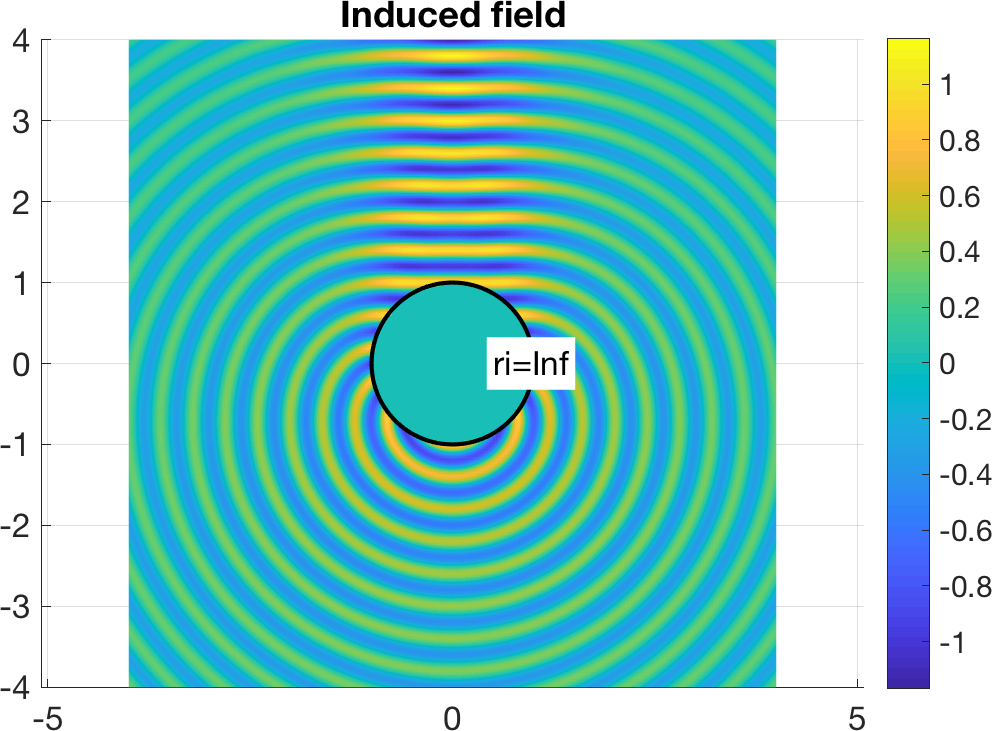
\includegraphics[width=5cm]{mie_example_soft_figure1.png}
    &
    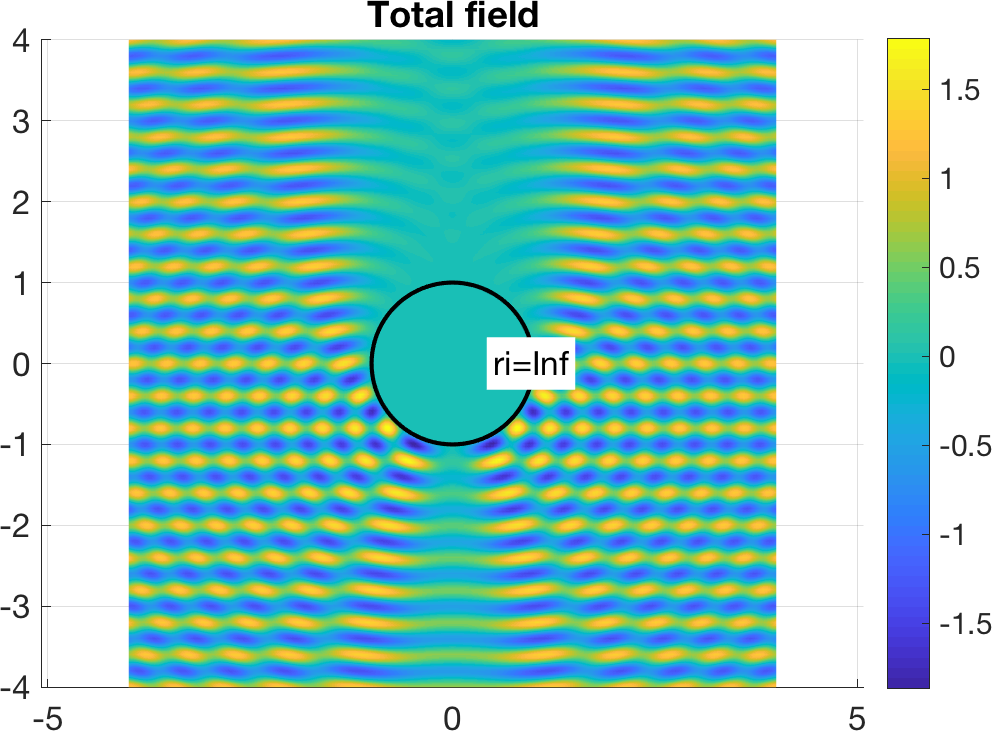
\includegraphics[width=5cm]{mie_example_soft_figure2.png}\\
    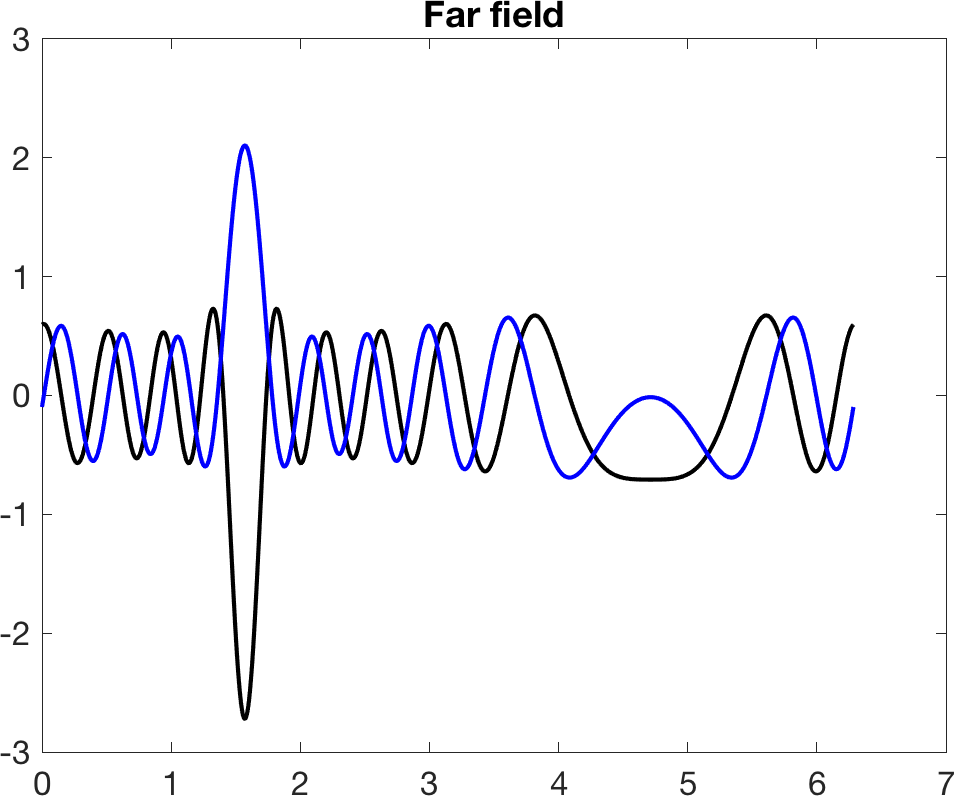
\includegraphics[width=5cm]{mie_example_soft_figure3.png}
    &
    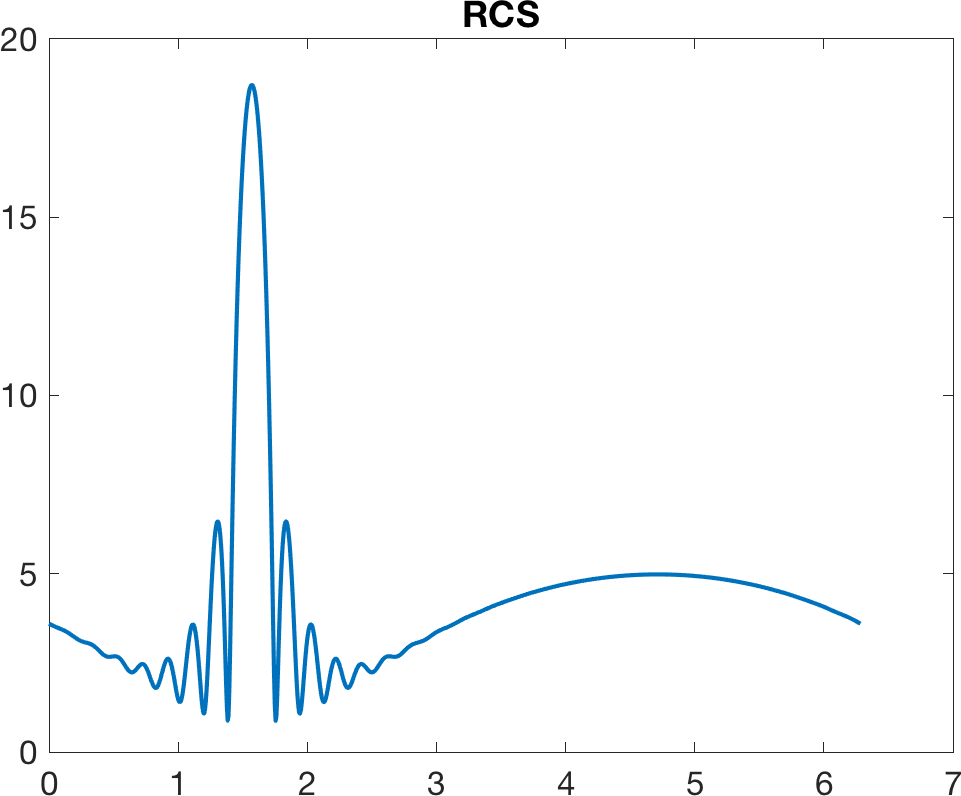
\includegraphics[width=5cm]{mie_example_soft_figure4.png}
  \end{tabular}
\end{center}

\techheading{Figures from \texttt{mie\_example\_hard}}
\begin{center}
  \begin{tabular}{cc}
    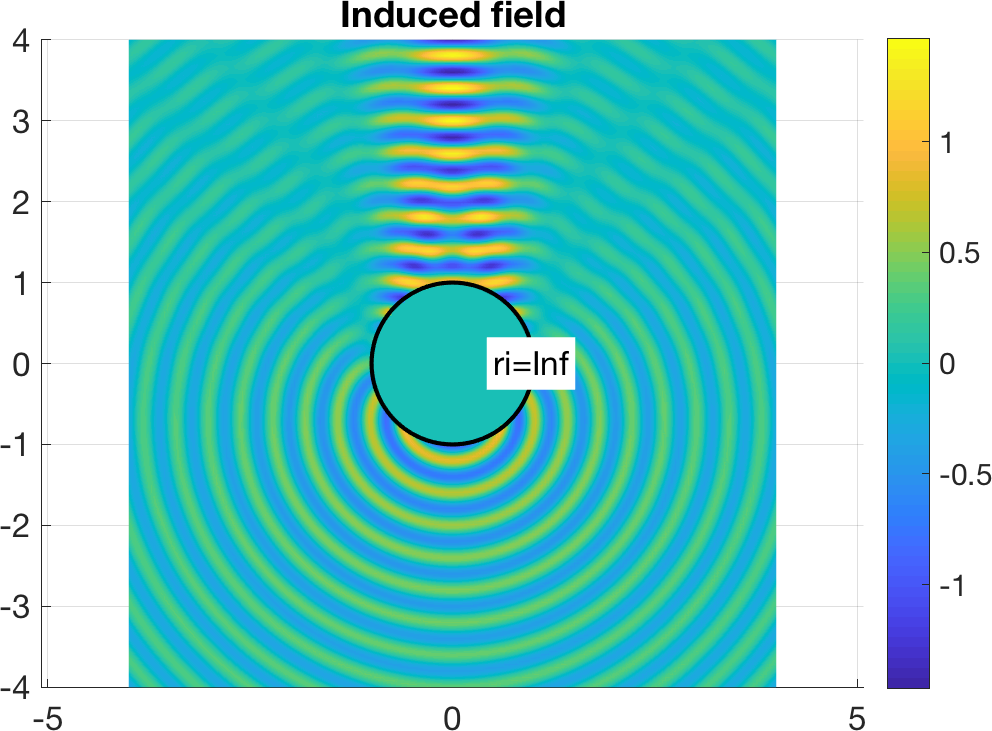
\includegraphics[width=5cm]{mie_example_hard_figure1.png}
    &
    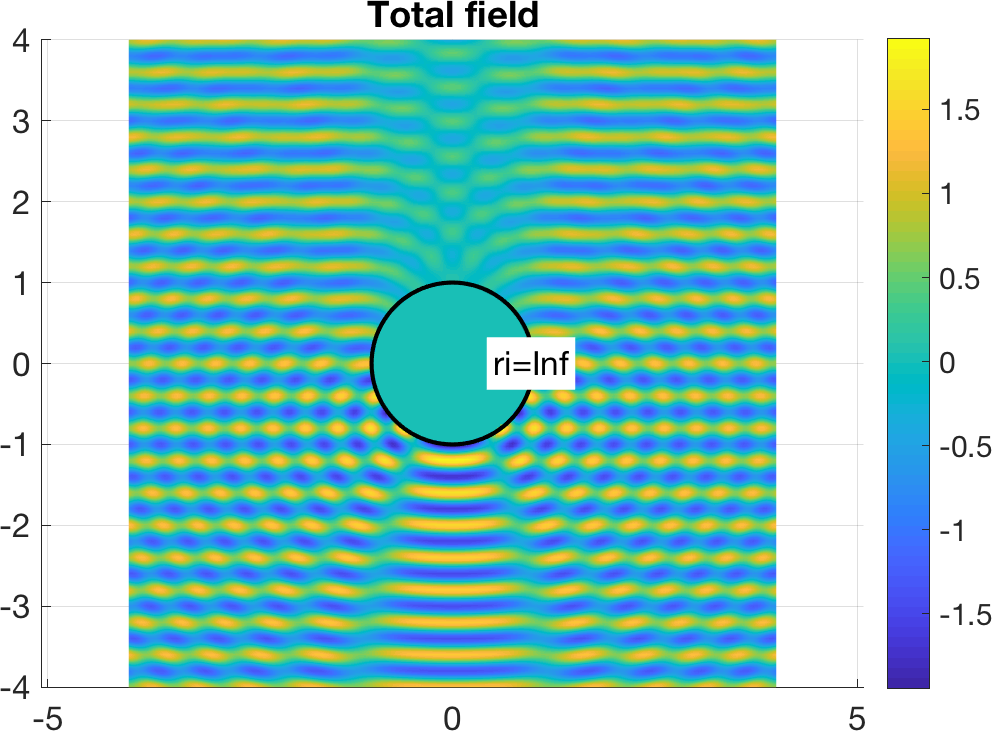
\includegraphics[width=5cm]{mie_example_hard_figure2.png}\\
    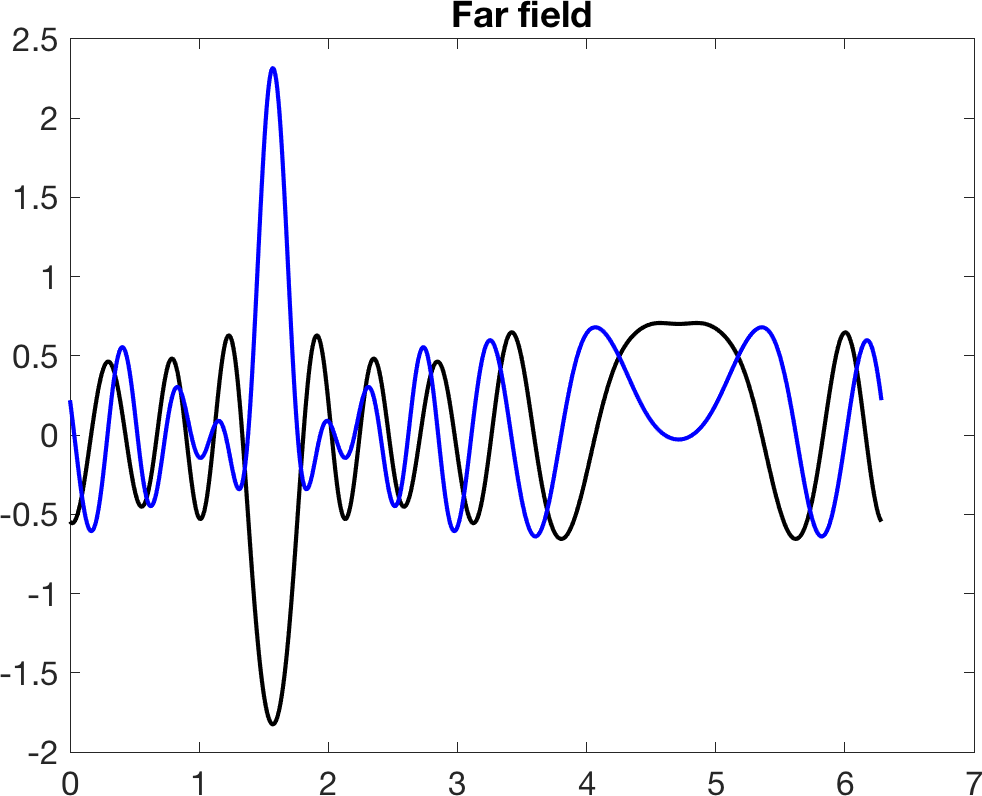
\includegraphics[width=5cm]{mie_example_hard_figure3.png}
    &
    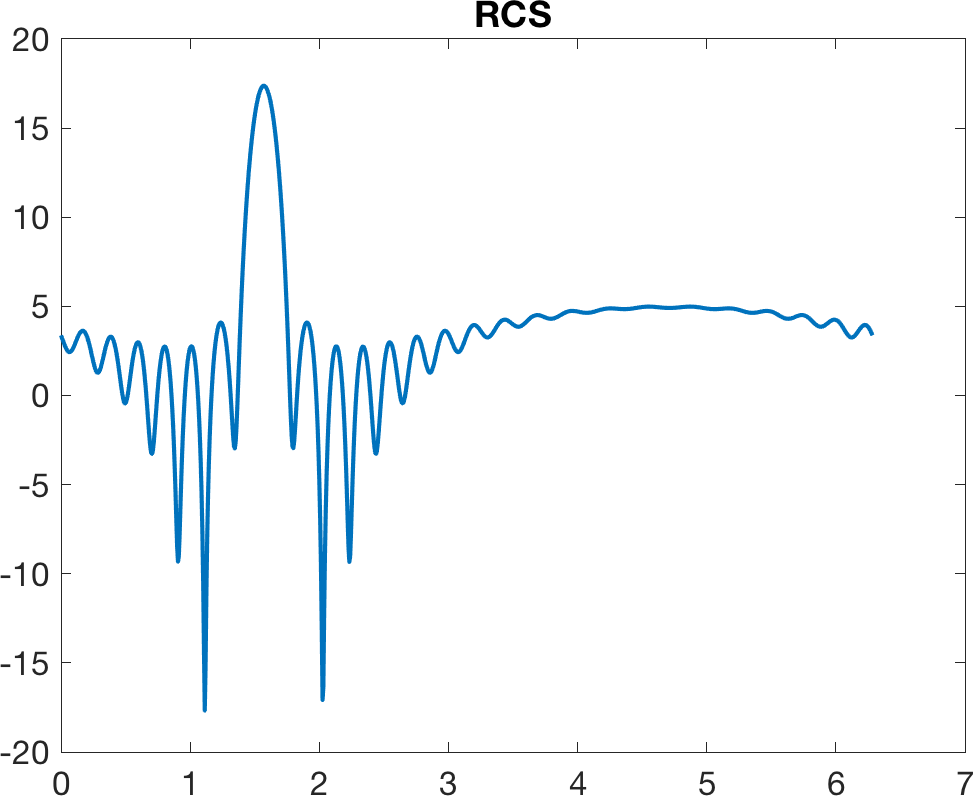
\includegraphics[width=5cm]{mie_example_hard_figure4.png}
  \end{tabular}
\end{center}

\newpage 
\techheading{Figures from \texttt{mie\_example\_robin}}
\begin{center}
  \begin{tabular}{cc}
    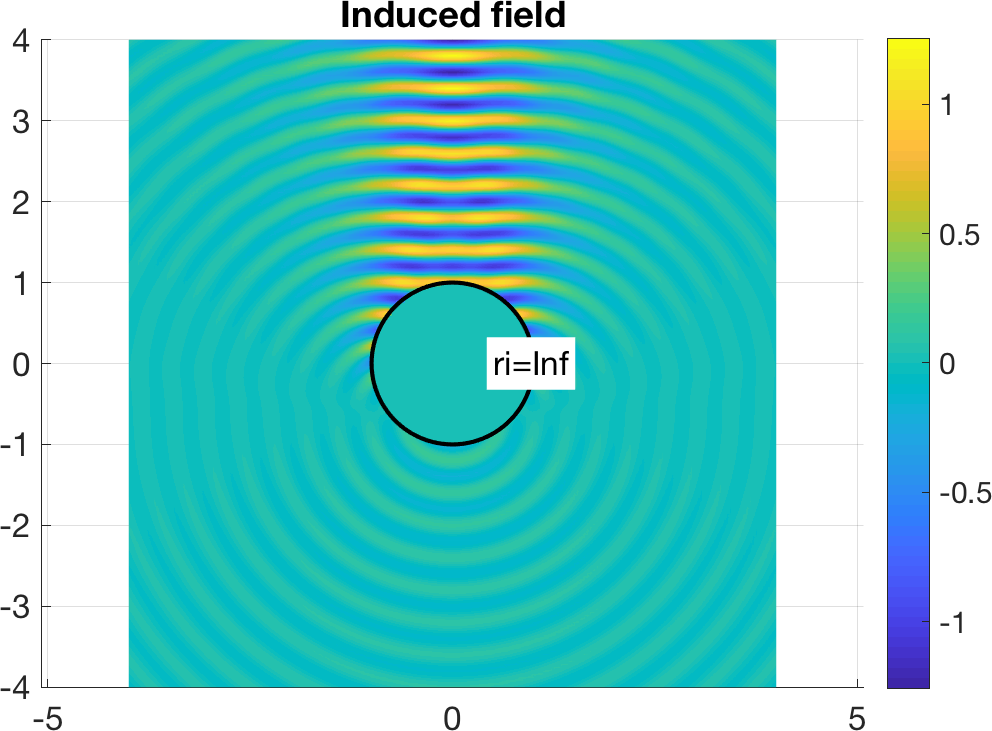
\includegraphics[width=5cm]{mie_example_robin_figure1.png}
    &
    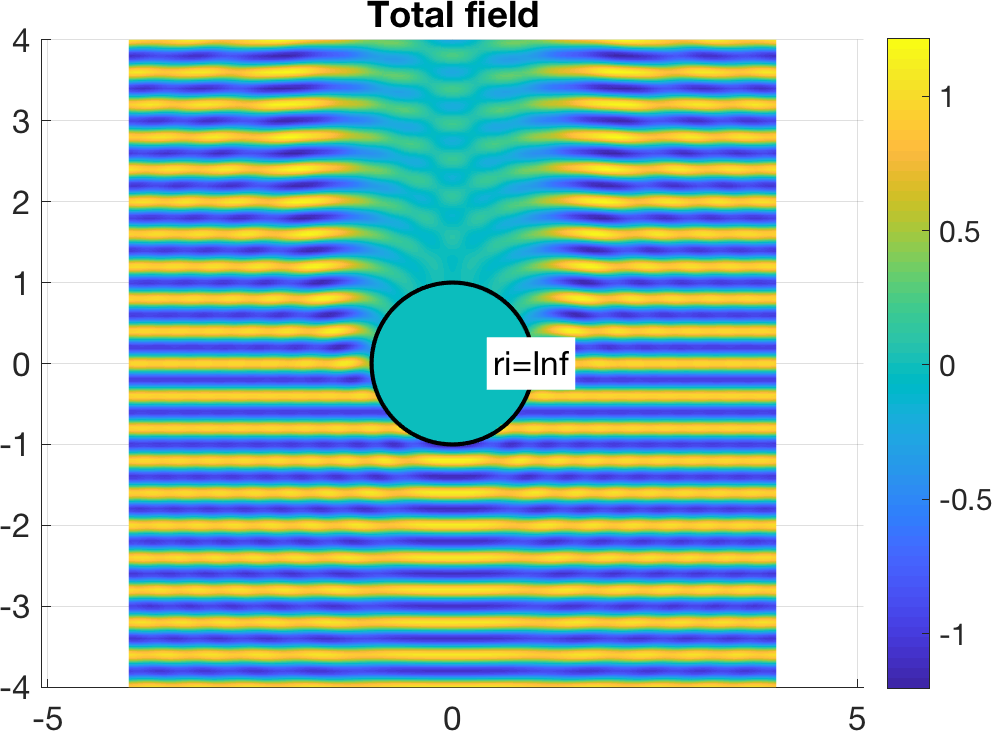
\includegraphics[width=5cm]{mie_example_robin_figure2.png}\\
    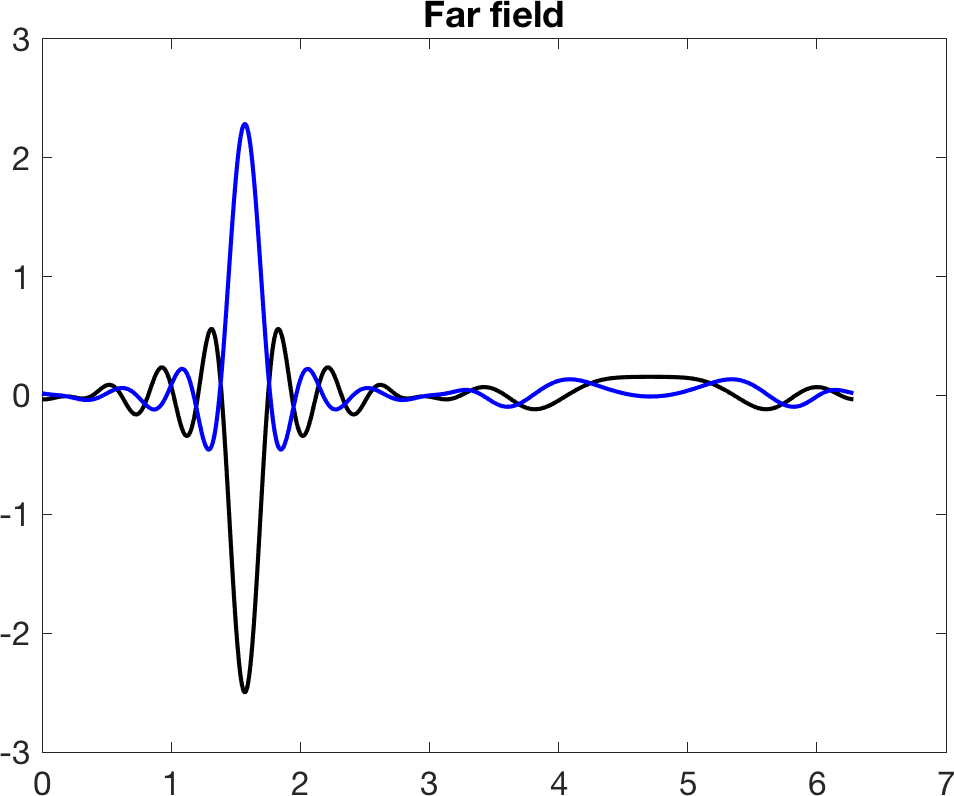
\includegraphics[width=5cm]{mie_example_robin_figure3.png}
    &
    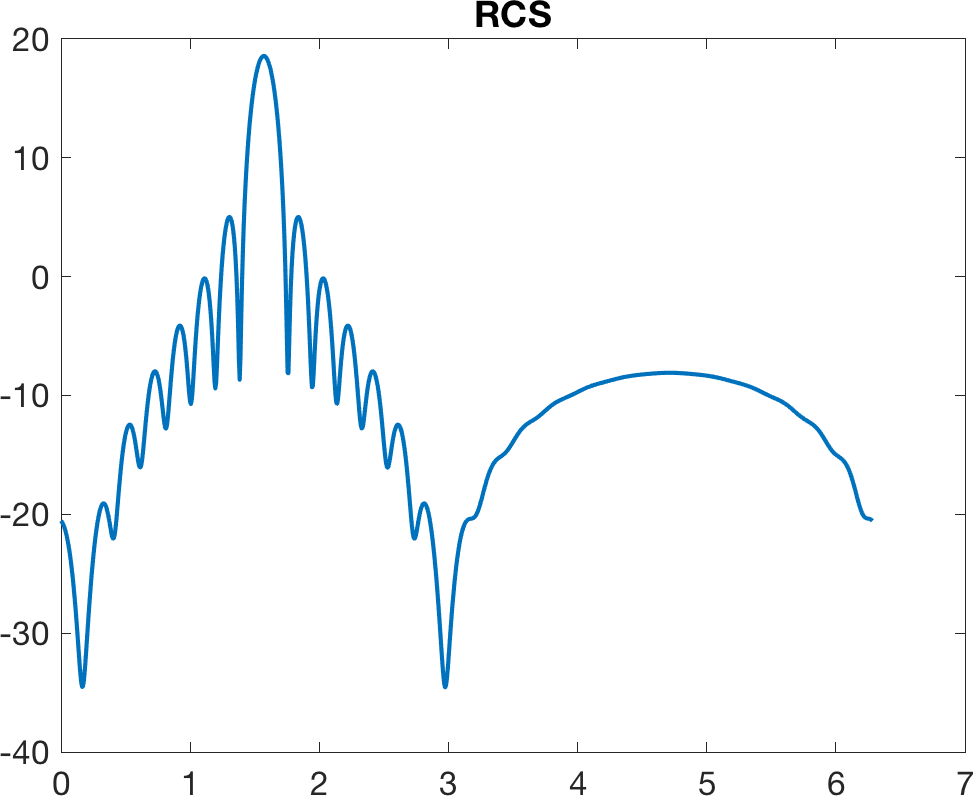
\includegraphics[width=5cm]{mie_example_robin_figure4.png}
  \end{tabular}
\end{center}

\techheading{Figures from \texttt{mie\_example\_coated}}
\begin{center}
  \begin{tabular}{cc}
    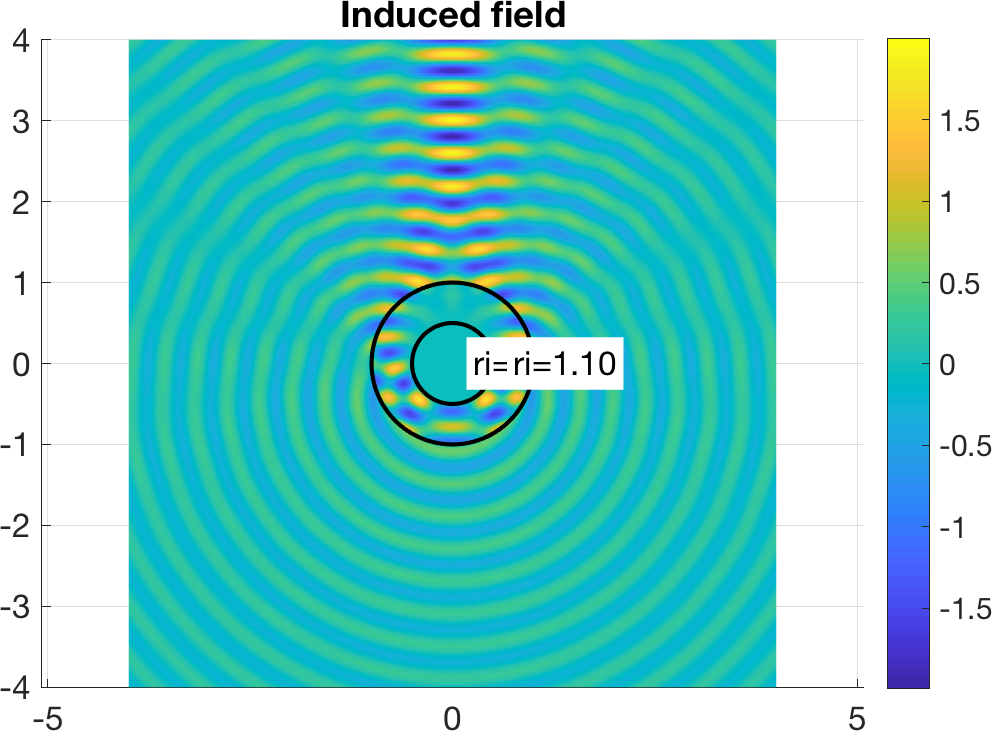
\includegraphics[width=5cm]{mie_example_coated_figure1.png}
    &
    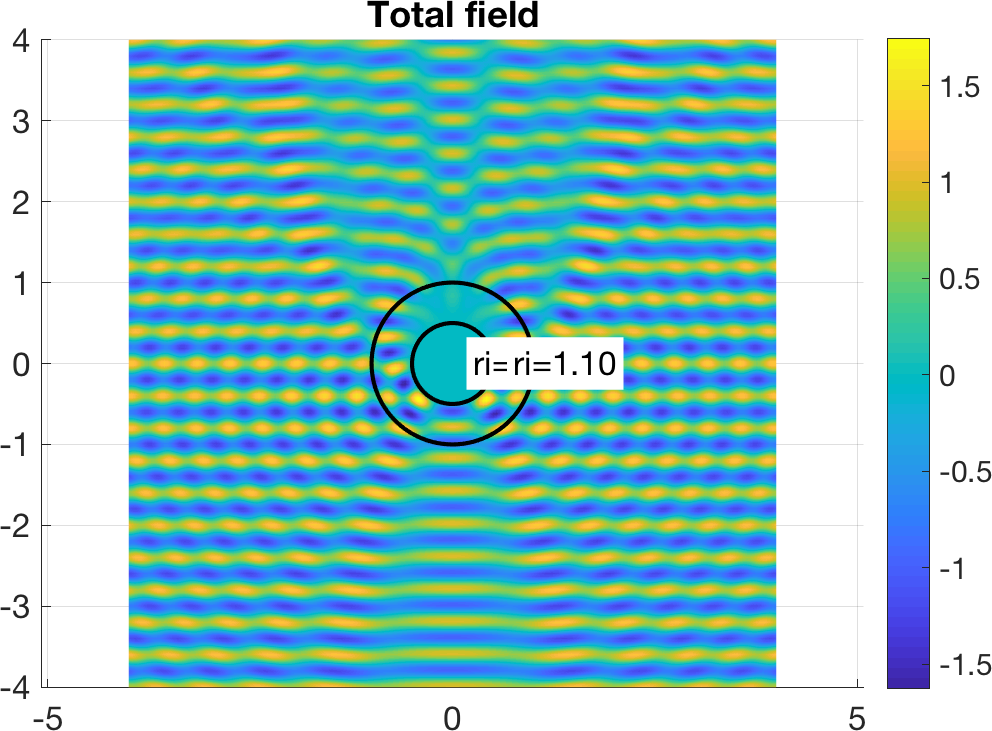
\includegraphics[width=5cm]{mie_example_coated_figure2.png}\\
    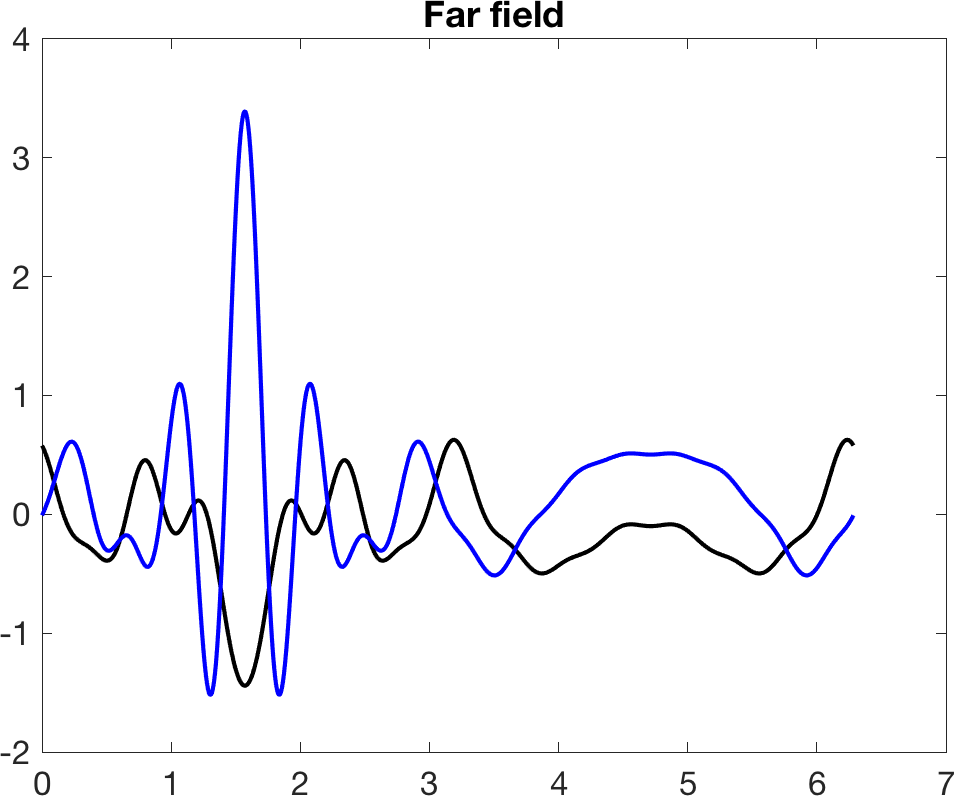
\includegraphics[width=5cm]{mie_example_coated_figure3.png}
    &
    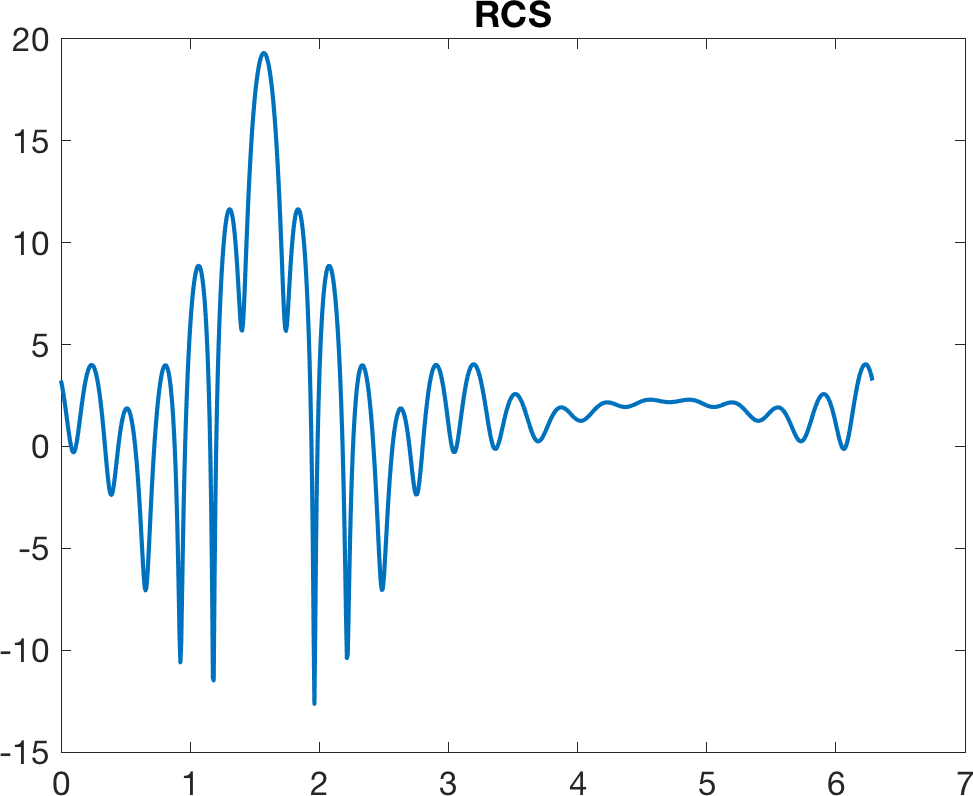
\includegraphics[width=5cm]{mie_example_coated_figure4.png}
  \end{tabular}
\end{center}

\newpage 
\techheading{Figures from \texttt{mie\_example\_dielectric}}
\begin{center}
  \begin{tabular}{cc}
    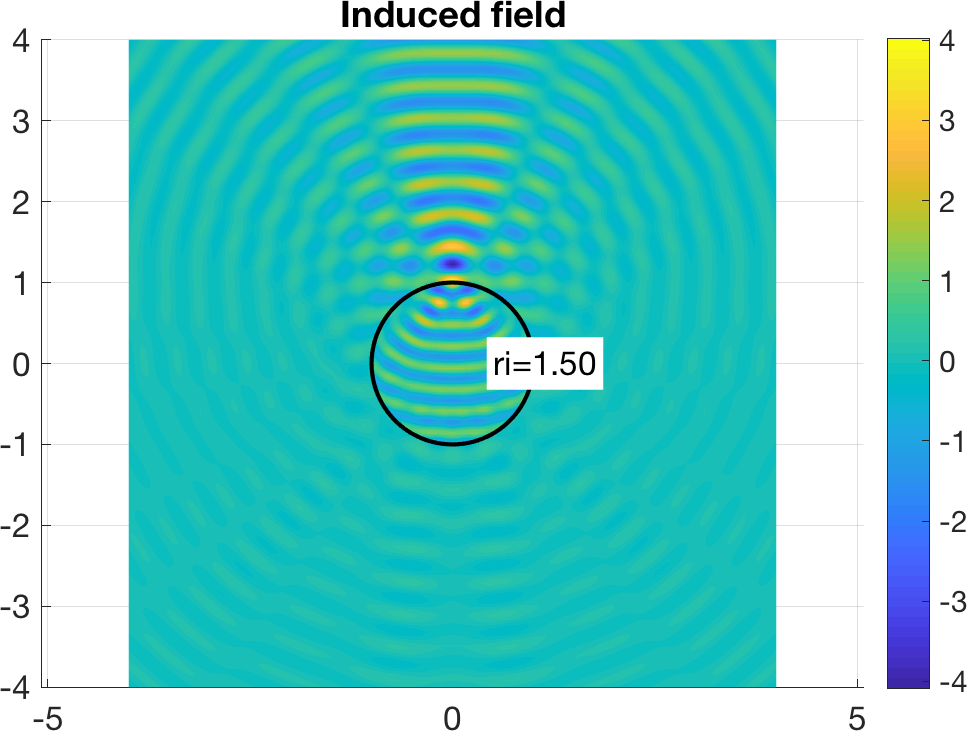
\includegraphics[width=5cm]{mie_example_dielectric_figure1.png}
    &
    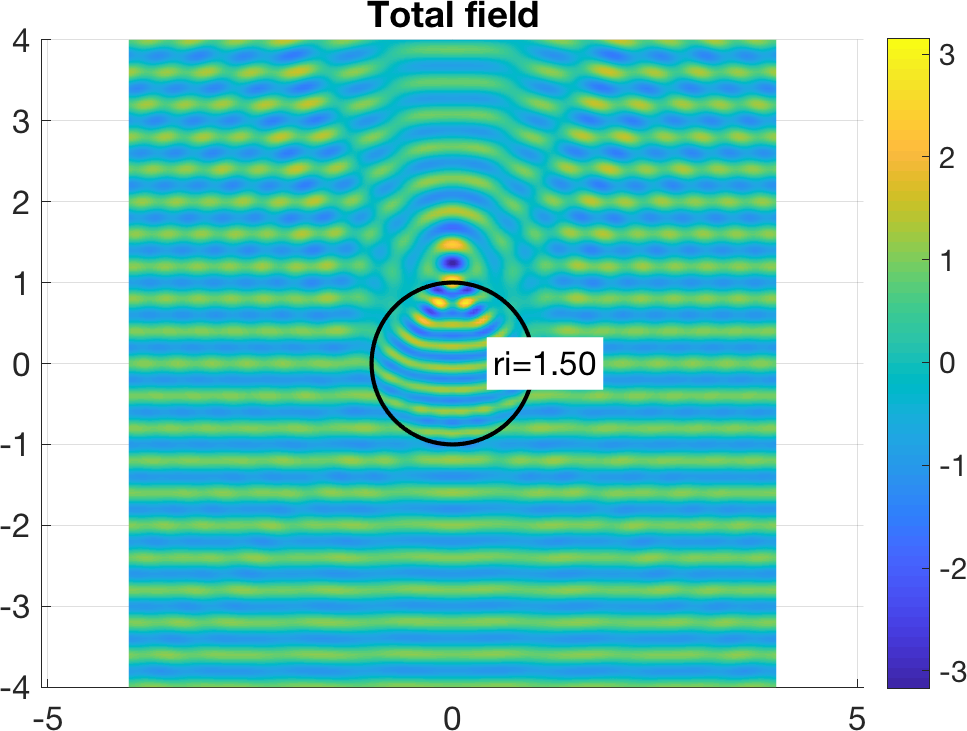
\includegraphics[width=5cm]{mie_example_dielectric_figure2.png}\\
    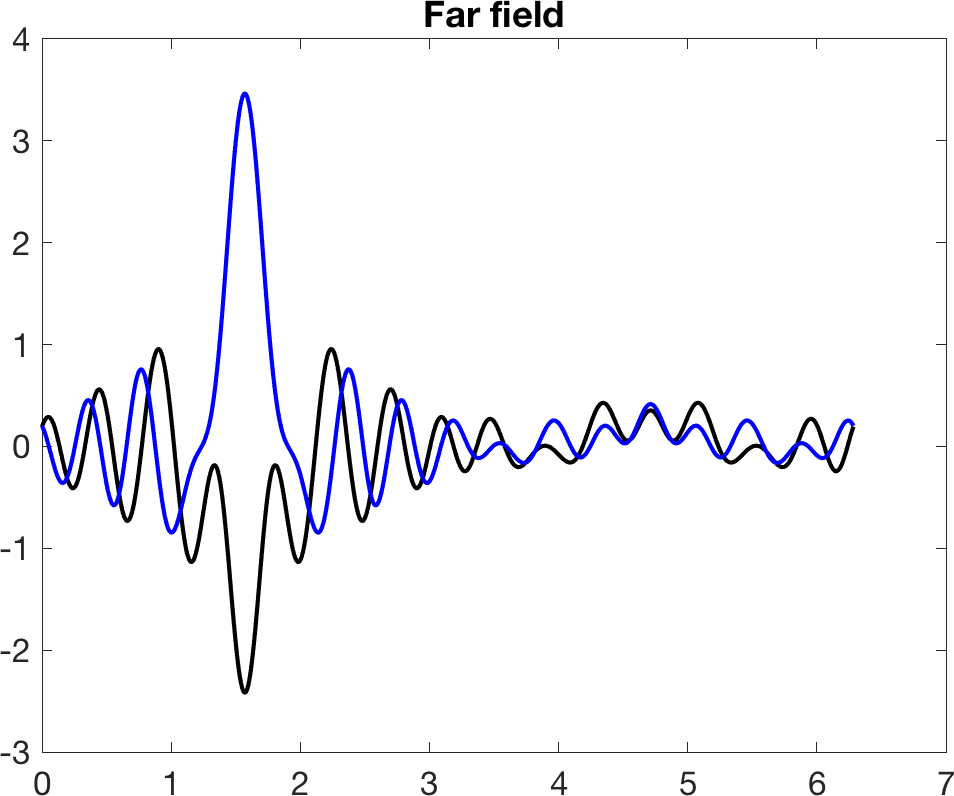
\includegraphics[width=5cm]{mie_example_dielectric_figure3.png}
    &
    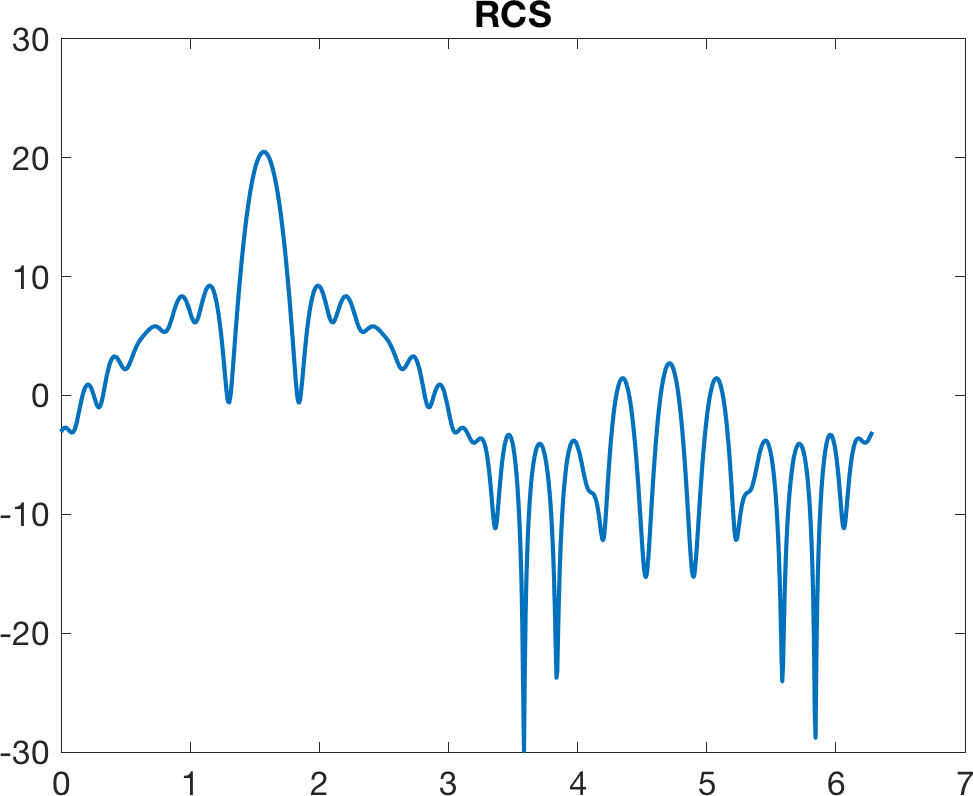
\includegraphics[width=5cm]{mie_example_dielectric_figure4.png}
  \end{tabular}
\end{center}


\end{document}
